\section{Deep Learning et Attention}
\subsection{Généralités}
\noindent \textbf{Attention}: Cette partie va se reposer sur des architectures avancées de Deep Learning. Afin de comprendre le contexte, il est nécessaire d'avoir une connaissance générale de l'architecture des \textit{Neural Machine Translation}, des \textit{Encoder-Decoder} (Section \ref{encoderDec}) et des réseaux récurrents (Section \ref{recarchi}), particulièrement les conventions d'écriture matricielle.\\

\noindent Pour réaliser une tâche, un réseau de neurones n'a pas nécessairement besoin de se focaliser sur l'intégralité de l'information pour produire sa décision. Par exemple, lorsqu'une traduction d'un texte est réalisée, le réseau doit se \textit{concentrer} sur le mot qu'il traduit et son contexte uniquement. Dans le cas contraire, le risque majeur est qu'il n'arrive pas à isoler la partie discriminante nécessaire à sa prédiction et de ce fait, que sa prédiction soit mauvaise.\\

\noindent Ce comportement est représentable en Deep Learning grâce au procédé nommé \textbf{Attention}. L'\textit{Attention} permet au réseau de se focaliser sur un sous-ensemble de l'information afin de mieux cibler l'information nécessaire à la tâche qu'il réalise. L'\textit{Attention} est responsable d'une amélioration significative des réseaux de neurones, notamment pour la traduction automatique où il apporte une solution élégante à la contrainte dimensionnelle du réseau traducteur. En effet, il a été montré que plus un texte est volumineux, plus le réseau se doit d'être volumineux\cite{malectrad}\cite{malectrad2}, ce qui est très problématique pour les contraintes matérielles actuelles. La qualité de la prédiction suit la courbe décrite par la Figure \ref{tradperf} lorsqu'un réseau de taille fixe voit la dimension de sa donnée d'entrée augmenter. L'\textit{Attention} permet de conserver une performance stable malgré l'augmentation de la dimension de la donnée d'entrée pour une architecture fixée et permet ainsi, de s'émanciper de la condition de proportionnalité entre dimension du réseau et dimension de l'entrée.\\

\begin{figure}
    \centering
    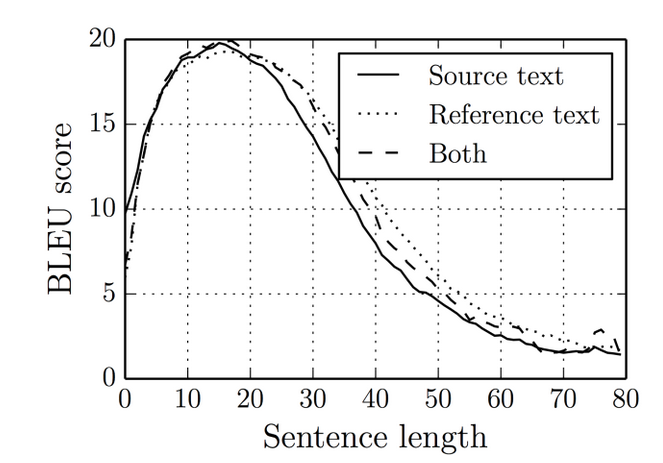
\includegraphics[scale=0.3]{./tex/attention-deep-learning/curveatt.png}
    \caption{Performance de la traduction selon la dimension du texte d'entrée}
    \label{tradperf}
\end{figure}

\noindent Formellement, l'\textit{Attention} consiste à construire dynamiquement une \textit{information de contexte} (noté $c(t)$) à partir d'un ensemble de contextes locaux issus d'une donnée source (notés $h_{i \in [1,n]}$). Ainsi, $c(t)=f \circ g(h_{i \in [1,n]}, q(t))$ avec f, fonction d'\textit{Attention}, g, fonction de proximité et q(t), contexte d'état auquel les différents contextes locaux sont comparés. La détermination de $c(t)$ peut être issue d'une approche déterministe ou probabiliste.\\

\noindent L'\textit{Attention} est un procédé très populaire depuis 2017 et voit son évolution rapide. Néanmoins, deux grandes familles d'architecture sont discernables: les approches \textit{Hard Attention} et \textit{Soft Attention}.

\subsection{Soft Attention}
\label{softattention}
Les approches \textit{Soft Attention} (Figure \ref{softatt}) reposent sur une hypothèse déterministe qui exprime le \textit{vecteur de contexte} $c(t)$ sous la forme d'une somme pondérées des différents contextes locaux $h_{i \in [1,n]}$. Ainsi,
$$c(t)=\sum_{i=1}^n \alpha_i h_i$$
$$\alpha_j(t)=align(h_j,q(t))=\frac{exp(e_j)}{\sum_{j' \in [1,n]} exp(e_{j'})}$$
$$e_j=score(h_j,q(t))$$

\noindent Les coefficients $\alpha_i$ sont obtenus par application de la fonction \textit{Softmax} afin de normaliser leurs valeurs et de rendre possible leurs interprétations probabilistes. La fonction \textit{score(.)} est la fonction qui évalue la proximité entre le vecteur référence et les contextes locaux. De nombreuses méthodes\footnote{Nous en étudierons certaines par la suite} ont été proposées à ce jour.\\

\noindent Cette méthode est différenciable. De ce fait, le mécanisme d'\textit{Attention} apprend par \textit{rétropropagation du gradient} comme le reste du réseau. Elle est donc évolutive, souple et permet une approche \textit{End-To-End}. Néanmoins, son impact sur le temps d'apprentissage est non négligeable. De plus, son hypothèse initiale impose que l'\textit{Attention} puisse être convenablement représentée par une combinaison linéaire. Du fait de sa simplicité d'apprentissage et d'implémentation, \textit{Soft Attention} est plus répandue que \textit{Hard Attention}. Néanmoins, les performances sont variables selon les données exploitées.

\begin{figure}
    \centering
    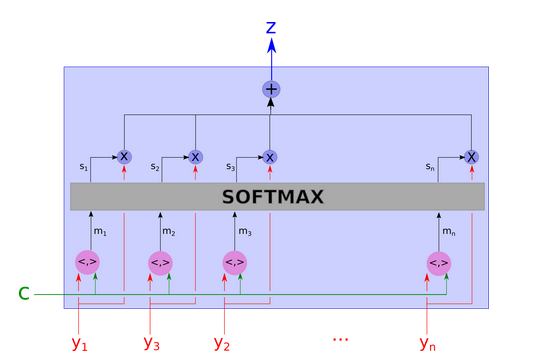
\includegraphics[scale=0.4]{./tex/attention-deep-learning/soft.png}
    \caption{Schématisation de l'approche Soft Attention}
    \label{softatt}
\end{figure}

\subsubsection{Fonction de proximité}
La fonction de proximité, appelée \textit{fonction d'alignement}, permet de calculer la proximité entre le vecteur référence et les différents contextes locaux. De nombreuses méthodes sont proposées mais les plus répandues sont:\\
\begin{enumerate}
    \item \textbf{Produit scalaire}: $score(h_j,q(t))=h_j^Tq(t)$
    \item \textbf{Produit scalaire pondéré}: $score(h_j,q(t))=h_j^TW_aq(t)$
    \item \textbf{Produit scalaire normé}\cite{attentionallneed}\footnote{Le facteur de normalisation est pertinent en cas de données à forte dimension afin de limiter l'impact d'un gradient faible, ce qui est nuisible à l'apprentissage}: $score(h_j,q(t))=\frac{h_j^Tq(t)}{\sqrt{n}}$
    \item \textbf{Couche Feed-Forward}\footnote{$v_c^T$ est utilisé afin d'obtenir une valeur unitaire}: $score(h_j,q(t))=v_c^Ttanh(W_c[h_j;q(t)])$
\end{enumerate}
\subsection{Hard Attention}
Les approches \textit{Hard Attention} (Figure \ref{hardatt}) reposent sur une méthode de \textit{sampling} stochastique. De ce fait, elles sont probabilistes. Ces approches extraient un \footnote{Voire deux parfois selon la méthode} vecteur local selon une densité de probabilités.  Ainsi $Z_i \sim h_i, \alpha_i$. \\

\noindent Du fait de son hypothèse initiale, les valeurs des gradients sont estimées par des \textit{méthodes de Monte-Carlo} et ne peuvent exploiter les gradients rétropropagés car non dérivables. Les méthodes \textit{Hard Attention} sont donc plus difficiles à implémenter et à exploiter au sein du réseau neuronal. L'\textit{Apprentissage par Renforcement} est très utilisé dans le cadre de ce type d'approches. Sur la Figure \ref{birdatt}, nous pouvons observer le comportement général des deux types d'\textit{Attention}. Alors que \textit{Soft Attention} a une focalisation diffuse caractéristique d'une somme pondérée, \textit{Hard Attention} se focalise sur une zone spécifique due à la sélection unitaire d'un contexte local. Ce type d'approche est moins exigeant en temps de calculs, ce qui la rend utile pour les tâches temps-réel.

\begin{figure}
    \centering
    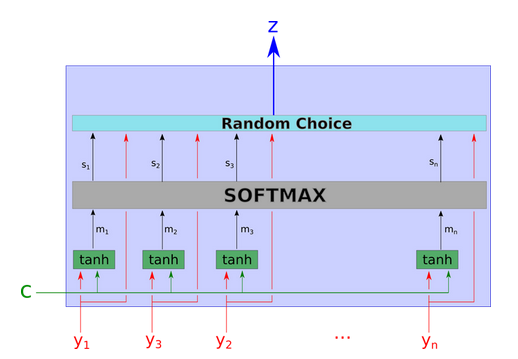
\includegraphics[scale=0.4]{./tex/attention-deep-learning/hard.png}
    \caption{Schématisation de l'approche Hard Attention}
    \label{hardatt}
\end{figure}

\begin{figure}
    \centering
    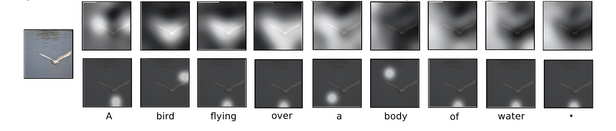
\includegraphics[scale=0.4]{./tex/attention-deep-learning/attbird.png}
    \caption{Visualisation du comportement de Soft Attention et Hard Attention}
    \label{birdatt}
\end{figure}


\subsection{Réseaux récurrents}
Un réseau récurrent est caractérisé par une structure temporelle où la mémoire conservée d'un évènement x à l'instant t tend à diminuer lorsque t augmente. De même, la projection\footnote{En exploitant l'état caché des cellules du RNN} d'une séquence dans un espace de dimension $R^d$ impose une destruction d'informations qui peut être critique pour la conservation de son contexte. Pour palier à ce défaut, une méthode simpliste (LSTM Bidirectionnelle) a été de lire les données temporelles pour t croissant et t décroissant. Néanmoins, cette solution favorise grandement les données en début de séquence et en fin de séquence. Pour les séries de grande dimension typique des textes, cette méthode est insuffisante pour garantir une prédiction de qualité. L'exploitation de l'\textit{Attention} est, à ce jour, la solution la plus performante pour combler cette problématique (Figure \ref{recatt}).

\begin{figure}
    \centering
    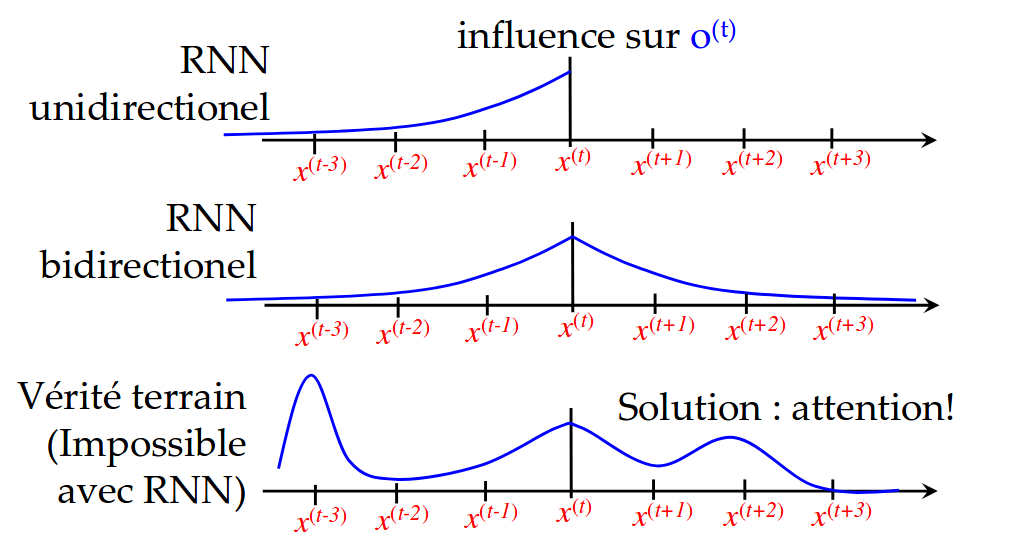
\includegraphics[scale=0.3]{./tex/attention-deep-learning/attentionlstm.png}
    \caption{Attention et réseaux récurrents}
    \label{recatt}
\end{figure}

\subsubsection{Approche Bahdanau}

L'architecture d'\textit{Attention} selon \textit{Bahdanau}\cite{softbadha} est une méthode de \textit{Soft Attention} démocratisée dans le cadre des \textit{Neural Machine Translation}. Ainsi, les vecteurs de contexte locaux correspondent aux sorties intermédiaires de l'Encoder et le vecteur référence correspond à l'état caché à l'instant t du Decoder.\\

\noindent L'approche Bahdanau repose sur l'architecture standard d'un NMT. Ainsi, contrairement à une cellule RNN classique qui considère uniquement l'état caché précédent et l'entrée actuelle, une cellule associée à l'\textit{Attention} selon Bahdanau recevra, en plus, un vecteur de contexte $c(t)$ \textbf{dynamiquement déterminé}\footnote{Dans un NMT classique, le vecteur de contexte est fixe et correspond au dernier état caché de l'Encoder.}. La méthode de détermination du vecteur de contexte $c(t)$ est identique à celle décrite dans la partie \ref{softattention}. Ainsi, nous avons:

$$h_{i, classic}=\phi_\theta(h_{i-1}, x_i)$$
$$h_{i, bahdanau}=\phi_\theta(h_{i-1}, x_i, c_i)$$

\noindent Afin d'uniformiser l'entrée, il est nécessaire de ramener à deux entrées uniquement. La méthode traditionnelle est de concaténer deux entrées afin de former un unique vecteur. Néanmoins, l'approche est peu détaillée dans les articles de recherche et le choix des vecteurs est variable selon les sensibilités de chacun.\\

\noindent Ce mécanisme est illustré sur la Figure \ref{bahdanau}. On peut constater que l'attention appliquée à l'instant t est calculé à partir de l'état caché précédent soit à l'instant t-1. Il n'y a donc pas de considération de l'état actuel (donc du dernier mot à l'entrée du réseau) pour déterminer le contexte.

\begin{figure}
    \centering
    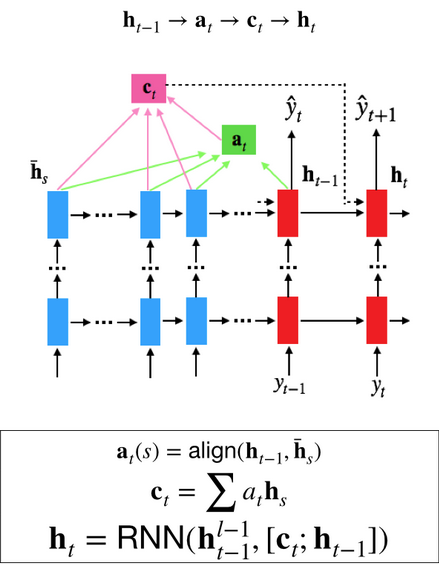
\includegraphics[scale=0.4]{./tex/attention-deep-learning/badhanaupic.png}
    \caption{Attention selon Bahdanau}
    \label{bahdanau}
\end{figure}

\subsubsection{Approche Luong}

\noindent L'architecture d'\textit{Attention} selon \textit{Luong}\cite{softluong} est très similaire à l'approche \textit{Bahdanau}. La spécificité se situe au niveau de la relation entre le vecteur de contexte et l'état caché du Decoder du réseau dans le cadre de la prédiction de la sortie.\\

\noindent Supposons un \textit{Neural Machine Translation}. Nous définissons $\hat{h}_s$, vecteurs de contexte locaux issus de l'Encoder et $h_t$, vecteur de référence défini par l'état caché du Decoder à l'instant t. Le vecteur $c(t)$ est le vecteur de contexte obtenu par la somme des vecteurs $\hat{h}_s$ pondérés par les poids d'attention $\alpha_s$.\\

\noindent Supposons $y_t$, prédiction du réseau à l'instant t soit un mot dans le cadre d'un NMT. Dans son architecture standard, $y_t=softmax(W_{dict}h_t)$. L'approche Luong rajoute une couche Full-Connected entre la sortie $h_t$ et $y_t$ qui appliquera l'attention. Ainsi:
$$y_t=softmax(W_{dict}\tilde{h}_t)$$
$$\tilde{h}_t=tanh(W_c[c_t;h_t])$$

\noindent Ce mécanisme est illustré sur la Figure \ref{luong}. On peut constater que l'attention appliquée à l'instant t est calculé à partir de l'état caché actuel soit à l'instant t. Il y a donc considération de l'état actuel, i.e le dernier mot en entrée du réseau, pour déterminer le contexte.

\begin{figure}
    \centering
    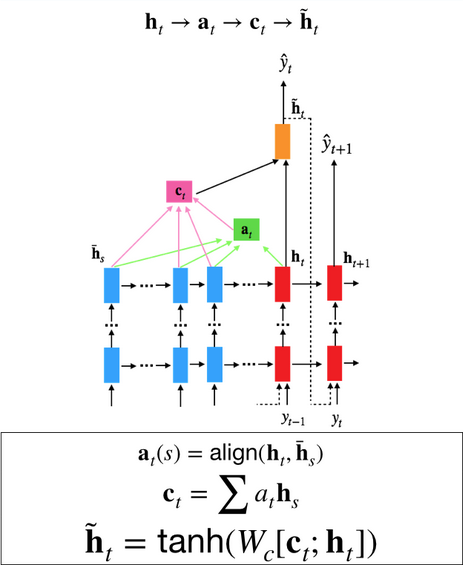
\includegraphics[scale=0.4]{./tex/attention-deep-learning/luongpic.png}
    \caption{Attention selon Luong}
    \label{luong}
\end{figure}

\paragraph{Attention globale et locale}
L'\textit{Attention} est dite \textit{globale} lorsqu'elle exploite l'intégralité des vecteurs de contexte. Dans le cadre de vecteurs de grande dimension et/ou de séquences de données de grande taille, la contrainte calculatoire peut être trop importante pour permettre l'exploitation de cette approche, notamment pour le (quasi) temps-réel comme la traduction automatique.\\

\noindent Au contraire, l'\textit{Attention} \textit{locale} constitue un compromis entre \textit{Soft Attention} (tous les vecteurs) et \textit{Hard Attention} (un seul vecteur) en ne considérant qu'un sous-ensemble des vecteurs de contexte. Ainsi:
$$c(t)=\phi_\theta(\hat{h}_{i,i \in [p_t-D;p_t+D]})$$ avec D, hyperparamètre défini empiriquement\footnote{Cette détermination peut être dure à réaliser et constitue une faiblesse importante de cette méthode} et $p_t$, référenciel inféré par le modèle pour chaque mot en entrée du Decoder.\\

\noindent \textit{Luong} propose deux approches pour déterminer $p_t$: l'approche \textit{monotonic} et \textit{predictive}.\\

\noindent L'approche \textit{monotonic} repose sur l'hypothèse que la position du mot-cible du Decoder est grossièrement alignée avec le mot source de l'Encoder. Ainsi, $p_t=t$ et constitue une constante du réseau. Cette méthode est assez peu efficace dans le cadre de la traduction automatique du fait des différences sémantiques et syntaxiques des langues.\\

\noindent L'approche \textit{predictive} apprend à prédire la position du référentiel afin de cibler le sous-ensemble le plus pertinent dans le cadre du mot-cible en entrée du Decoder. Supposons S, dimension de la séquence d'entrée du Decoder. Il est logique que $p_t$ soit dans $[0,S]$. Ainsi, nous avons:
$$p_t=S \cdot sigmoid(\varphi(h_t))$$
\noindent $\varphi$ est la fonction qui interprète l'état caché actuel pour définir la dimension de la fenêtre déterminée par $p_t$. Pour cela, une couche Full-Connected est utilisée. Nous obtenons donc:
$$\varphi(h_t)=v_p^Ttanh(W_ph_t)$$ avec $v_p$ et $W_p$, paramètres du modèle à inférer durant l'apprentissage.\\

\noindent Afin de favoriser l'alignement autour de $p_t$, les poids associés à l'\textit{Attention} sont modifiés. Ainsi, plus la position du mot est éloignée du référentiel, plus son importance sera diminuée\footnote{Néanmoins, un mot éloigné peut avoir un poids important si son alignement est très bon malgré une distance importante.}. Supposons $\alpha_i$, poids d'\textit{Attention} du i-ème vecteur de contexte local alors:
$$\alpha_t(j)=align(h_j,q(t)) \cdot exp(-\frac{(j-p_t)^2}{2\sigma^2})$$ avec $\sigma$ empiriquement défini à $\frac{D}{2}$, $p_t$ nombre réel et j, entier appartenant à la fenêtre centrée en $p_t$.



\subsubsection{Généralisation pour l'exploitation d'image: Image Captionning}
La notion d'\textit{Attention} est applicable à toute forme de données structurées. Ainsi, une image, un texte, un signal sonore ou même quelconque peuvent être exploités par une architecture exploitant l'\textit{Attention}. La différence se situe au niveau de la détemination des vecteurs de contexte obtenue par le réseau extracteur.\\

\noindent Dans le cas d'un réseau récurrent exploité comme extracteur (notamment pour les \textit{Neural Machine Translation}, les vecteurs de contexte peuvent être associés aux vecteurs d'états cachés des cellules RNN\footnote{Ou LSTM, GRU...}. Néanmoins, dans la cas d'un réseau convolutif (exploité pour l'\textit{Image Captionning} par exemple), il n'y a pas de "structure vectorielle" explicite. Il est donc nécessaire de proposer une méthode d'isolation des différents vecteurs de contexte.\\

\noindent Une image, à travers un réseau convolutif, est explicitée à travers les \textit{feature map} crées par les couches de convolution. De ce fait, l'information d'une image conserve la structure de la donnée initiale soit une forme matricielle. Une sortie d'une couche convolutive est un ensemble de \textit{feature map}. Une même localisation spatiale sur les différentes \textit{feature map} correspond à un résultat d'analyse d'une même partie spatiale de la donnée en amont. De ce fait, elles sont associées à une même entité alors que deux localisations distinctes sur une même \textit{feature map} correspond à deux analyses de deux parties distinctes de l'image en amont. \\

\noindent Cette spécificité permet d'isoler la structure vectorielle nécessaire à la création des vecteurs de contexte. Supposons une sortie d'une couche de convolution de profondeur D et dont les \textit{feature map} sont \textit{carrés}. Nous avons donc une sortie de la forme M*M*D. Nous obtenons ainsi M*M vecteur de contexte de dimension D. Cette séparation permet ainsi de \textit{découper} une image en un ensemble de vecteurs représentatifs de ses caractéristiques. Une contrainte importante est le \textit{choix} de la couche convolutive à exploiter\footnote{Il est logique de favoriser les dernières couches avec un haut pouvoir d'abstraction}. Le même comportement est applicable sur un signal quelconque car le comportement des \textit{feature map} est indépendant de la nature de la donnée d'entrée. La Figure \ref{capim} illustre cette approche.

\begin{figure}
    \centering
    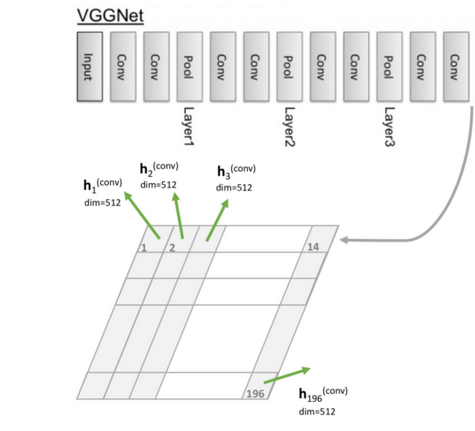
\includegraphics[scale=0.3]{./tex/attention-deep-learning/capim.png}\\
    La dimension du vecteur de contexte est 512 car la profondeur de la sortie de la 4ième couche d'un réseau VGGNet est de 512. La valeur est différente selon le réseau et la couche convolutive exploitée.
    \caption{Extraction des vecteurs de contexte à partir d'une feature map}
    \label{capim}
\end{figure}


\subsection{Réseaux convolutifs}
\noindent L'\textit{Attention} a été popularisée grâce à sa gestion des \textit{vecteurs de contexte}. Cependant, il est possible d'appliquer ses concepts sur d'autres architectures neuronales, notamment les réseaux convolutifs.\\

\noindent Dans le cadre des RNN, les entités porteuses d'informations sont les vecteurs de contextes obtenus par les prédictions de cellules (souvent LSTM ou GRU) du réseau. L'équivalent dans un réseau convolutif sont les \textit{feature map} obtenues en sortie des couches de convolution. Appliquer l'\textit{Attention} à ce type de réseau revient donc à pondérer l'importance de chacune des \textit{feature map} produites durant l'apprentissage.

\subsubsection{Spatial Transformer}
Les données d'apprentissage (et à prédire) peuvent présenter des particularités géométriques variables. Ainsi, l'entité discriminante peut être décentrée au fil des images, son alignement peut être variable selon un angle $\theta$ ou encore, être représentée à une profondeur variable par rapport au référentiel du cadre de l'image (premier plan et second plan par exemple). Cette variabilité pose de grande difficulté d'apprentissage au modèle tout en forçant l'augmentation de sa complexité pour considérer les géométries variables des images. Afin de résoudre cette problématique, \textit{Spatial Transformer}\cite{standspa} (STN) propose une approche élégante.\\

\noindent Au lieu de traiter les données \textit{brutes}, \textit{Spatial Transformer} va réaliser une transformation géométrique de la donnée d'entrée (i.e \textit{feature map}) afin de la standardiser. Il réalise donc une action comparable à un pré-traitement qui facilite grandement le travail de discrimination du modèle. Ce module n'a que peu d'impact sur la vélocité du modèle.\\

\noindent Son comportement peut être grossièrement comparé à l'action d'une couche de Pooling. Néanmoins, \textit{Spatial Transformer} possède des avantages qui rend cette approche bien plus robuste. En effet, elle est:
\begin{itemize}
    \item \textbf{Modulable}: Elle est applicable à toute architecture avec facilité.
    \item \textbf{Apprenante}: Elle peut être entraînée par rétropropagation du gradient. Son utilisation garantit donc l'aspect End-To-End du réseau.
    \item \textbf{Evolutive}: La transformation réalisée par STN est dynamique selon la donnée d'entrée. Son comportement est donc adaptatif et bien plus robuste qu'une approche statique comme le Pooling par exemple.
\end{itemize}

\paragraph{Transformation d'image}
Afin de comprendre le fonctionnement du STN, la notion de \textit{transformation linéaire} doit être abordée.\\

\noindent Supposons un point X de coordonnées (x,y). Matriciellement, les coordonnées peuvent ainsi être décrites par:
$$X=\begin{bmatrix}
x \\
y
\end{bmatrix}$$

\noindent Soit M, une matrice 2*2 définie par:
$$M=\begin{bmatrix}
a & b \\
c & d
\end{bmatrix}$$

\noindent La transformation linéaire T est définie par la matrice $X'= T(X) = MX$.\\

\noindent Ainsi, supposons:
$$M=\begin{bmatrix}
1 & 0 \\
0 & 1
\end{bmatrix}$$
\noindent Alors:
$$X'=\begin{bmatrix}
1 & 0 \\
0 & 1
\end{bmatrix}\begin{bmatrix}
x \\
y
\end{bmatrix}=\begin{bmatrix}
x \\
y
\end{bmatrix}=X$$

\noindent Nous pouvons observer que la transformation réalisée est la \textit{transformation identité}. En modifiant les valeurs de la matrice M, nous pouvons réaliser différentes transformations du vecteur représenté par la matrice X. Ainsi, par exemple:
$$Scaling\footnote{On parle d'\textit{isotropic scaling} lorsqu'un même coefficient k est appliqué sur chaque dimension du vecteur.}: \ X'=\begin{bmatrix}
p & 0 \\
0 & q
\end{bmatrix}\begin{bmatrix}
x \\
y
\end{bmatrix}=\begin{bmatrix}
px \\
qy
\end{bmatrix}$$
$$Rotation: \ X' =  \begin{bmatrix}
\cos{\theta} & -\sin{\theta} \\
\sin{\theta} & \cos{\theta}
\end{bmatrix}
%
\begin{bmatrix}
x \\
y
\end{bmatrix} =
\begin{bmatrix}
x\cos{\theta}- y\sin{\theta} \\
x\sin{\theta} + y\cos{\theta}
\end{bmatrix}$$

\noindent Il est possible de cumuler différentes transformations sur un même vecteur. Supposons 3 transformations définies par les matrices Q, R et S. Nous avons donc $X'=Q[R(SX)]=MK, \ M=QRS$.\\

\noindent \textbf{Attention}: L'ordre des transformations est significatif car le produit matriciel n'est pas une opération commutative\footnote{C'est à dire que $A*B \neq B*A$}!\\

\noindent Supposons que nous voulons réaliser une \textit{translation} vectorielle. Cette transformation pose problème car, avec le modèle décrit précédemment, chaque dimension du vecteur transformé correspond à une fonction linéaire des composantes du vecteur initial. Or, dans le cadre d'une translation, nous ne réalisons pas une transformation linéaire. La translation est une transformation standard et très exploitée. Corriger ce défaut est une nécessité dans le cadre du SNT.\\

\noindent Pour résoudre ce dilemme, une solution consiste à exploiter une nouvelle dimension de projection vectorielle pour représenter le vecteur à transformer. Ainsi, supposons X dans $R^2$ alors nous représenterons X dans $R^3$ tel que:
$$X=\begin{bmatrix}
x \\
y\\
1
\end{bmatrix}$$

\noindent De ce fait, nous pouvons construire une matrice représentant une transformation T telle que:
$$M=
\begin{bmatrix}
  a & b & 0 \\
  c & d & 0 \\
  0 & 0 & 1
\end{bmatrix}$$

\noindent Afin de réaliser une translation, nous effectuons donc:
$$X'=
\begin{bmatrix}
  a & 0 & e \\
  0 & d & f \\
  0 & 0 & 1
\end{bmatrix}\begin{bmatrix}
x \\
y\\
1
\end{bmatrix}=\begin{bmatrix}
ax+e \\
dy+f\\
1
\end{bmatrix}$$

\noindent Bien que fonctionnelle, cette approche impose la conservation de la troisième dimension qui ne sert que dans le cadre d'un jeu d'écriture. Afin de corriger ce défaut, il est nécessaire de modifier la matrice M. Supposons M telle que:
$$M=
\begin{bmatrix}
  a & 0 & e \\
  0 & d & f \\
\end{bmatrix}$$
\noindent Alors:
$$
X' =  \begin{bmatrix}
a & 0 & \Delta \\
0 & d & \Delta
\end{bmatrix}
%
\begin{bmatrix}
x \\
y \\
1
\end{bmatrix} =
\begin{bmatrix}
ax + \Delta \\
dy + \Delta
\end{bmatrix} $$
\noindent Nous observons que la translation selon $\Delta$ a bien été réalisée et que l'unicité des dimensions est respectée. Nous avons donc généralisée notre modèle de transformation en permettant la réalisation de \textit{transformations affines}.

\paragraph{Interpolation bilinéaire}
Le modèle décrit dans le pragraphe précédent permet la réalisation de transformation vectorielle via l'aide d'un produit matriciel. Néanmoins, la structure d'une image a une contrainte importante: les coordonnées doivent être entières car un pixel possède des coordonnées entières. Or, suite à une transformation, les coordonnées obtenues peuvent être décimales. Comment pouvons nous "cibler" le pixel correspondant à des coordonnées non entières ?\\

\noindent Pour résoudre ce problème, l'\textit{interpolation bilinéaire} est utilisée. Elle exploite les 4 pixels les plus proches afin de définir une valeur pour le pixel "abstrait". Le résultat est ainsi plus lisse et permet la création d'image plus réaliste.\\

\noindent Supposons un point P de coordonnées (x,y) et 4 points de références tels que $Q_{11} = (x_1, y_1)$, $Q_{21} = (x_2, y_1)$, $Q_{12} = (x_1, y_2)$, $Q_{22} = (x_2, y_2)$. Ces points sont représentés sur la Figure \ref{bilineaire}. \\

\noindent Schématiquement, nous pouvons considérer P comme un point présent sur la surface d'un carré dont les sommets sont pondérés par une valeur propre. Afin d'approximer P, il est donc nécessaire d'évaluer sa distance par rapport à chacun de ces sommets et de réaliser une moyenne pondérée de leurs valeurs selon les distances. Pour cela, nous définirons $R_1$ et $R_2$, comme intensité du pixel intermédiaire entre deux pixels successifs selon l'axe des abscisses. Par la suite, nous définirons l'intensité de P comme valeur d'une moyenne pondérée de $R_1$ et $R_2$. Cette approche permet donc de considérer la position spatiale de P et d'approximer sa valeur.\\

\noindent Nous définissons::
$$R_1 = \frac{x_2 - x}{x_2 - x_1}Q_{11} + \frac{x - x_1}{x_2 - x_1}Q_{21}$$
$$R_2 = \frac{x_2 - x}{x_2 - x_1}Q_{12} + \frac{x - x_1}{x_2 - x_1}Q_{22}$$
\noindent Et ainsi:
$$\boxed{P = \frac{y_2 - y}{y_2 - y_1}R_1 + \frac{y - y_1}{y_2 - y_1}R_2}$$

\begin{figure}
    \centering
    \begin{tabular}{cc}
    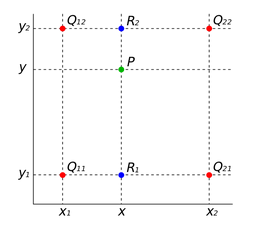
\includegraphics[scale=0.4]{./tex/attention-deep-learning/bilineaire.png} & 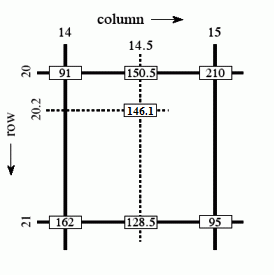
\includegraphics[scale=0.4]{./tex/attention-deep-learning/Bilin3.png} \\
    \end{tabular}
    \caption{Illustration de l'interpolation bilinéaire}
    \label{bilineaire}
\end{figure}

\paragraph{Le module SNT}
Afin de réaliser une transformation affine d'une image, 3 étapes sont nécessaires:
\begin{itemize}
    \item \textbf{Création du grille d'échantillonnage}: La grille est composée de vecteurs de coordonnées (x,y) telles que $x_{max},y_{max}$ égales aux dimensions de l'image initiale. En d'autres mots, il y a création d'un \textit{meshgrid} de même dimension que l'image initiale.
    \item \textbf{Application de la matrice de transformation}: La matrice de transformation est appliquée sur les différents vecteurs du \textit{meshgrid} obtenu lors de l'étape précédente.
    \item \textbf{Correction de la grille}: Afin de pouvoir obtenir une image valide, il est nécessaire de corriger les pixels "non entiers". Pour cela, une méthode d'interpolation est nécessaire.
\end{itemize}

\noindent Le module SNT est composé de deux parties: \textit{Localisation Network} et \textit{Grid generator}. Une illustration de son architecture est visible sur la Figure \ref{sntransf}.\\

\begin{figure}
    \centering
    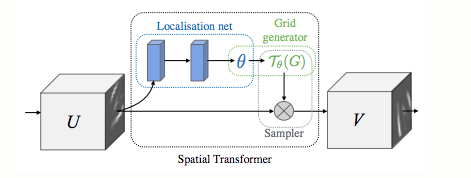
\includegraphics[scale=0.4]{./tex/attention-deep-learning/sntmod.png}
    \caption{Illustration du module SNT}
    \label{sntmod}
\end{figure}


\noindent L'objectif de \textit{Localisation Network} est de produire la matrice de transformation $\theta$, i.e une matrice (2,3)\footnote{Voir la partie précédente pour justifier l'utilisation d'une telle matrice.}. Pour cela, un réseau Full-Connected (ou éventuellement convolutif) est exploité. \\

\noindent Ce réseau reçoit la \textit{feature map} en entrée et il produit une sortie de dimension (6,) correspondant aux paramètres de la matrice de transformation. Ce modèle est capable d'apprentissage du fait de son architecture. Il apprend à réaliser la \textit{meilleure} transformation à appliquer sur une donnée d'entrée afin de favoriser la meilleure qualité prédictive. Il est \textbf{important} de comprendre que la transformation réalisée est dynamique et propre aux spécificités de la donnée d'entrée. Le module applique donc différentes transformations selon la donnée. Le modèle n'apprend donc pas à appliquer une transformation unique pour toutes les données mais quelle transformation réaliser selon la donnée. Bien que rien n'impose l'application d'une transformation particulière, nous avons observé expérimentalement que le comportement du réseau est comparable au comportement humain, i.e centrer l'entité discriminante et uniformiser son inclinaison selon les caractéristiques du jeu d'apprentissage. Par exemple, sur la Figure \ref{sntransf}, nous pouvons observer le type de transformation dans le cadre du jeu de données MNIST.\\

\begin{figure}
    \centering
    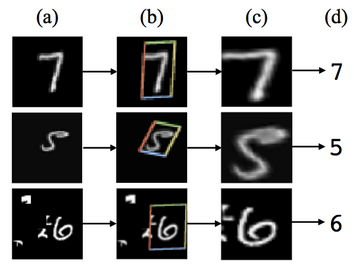
\includegraphics[scale=0.4]{./tex/attention-deep-learning/sntmnist.png}
    \caption{Illustration d'une transformation par SNT avec le dataset MNIST}
    \label{sntransf}
\end{figure}

\noindent La seconde partie correspond au \textit{Grid generator}. Il est chargé de réaliser la transformation affine de la donnée d'entrée selon la matrice de transformation obtenue par \textit{Localisation Network}.\\

\noindent En d'autres mots, il va produire le \textit{meshgrid} et réaliser le produit matriciel avec la matrice de transformation. Afin de permettre des transformations affines (et le produit matriciel avec une matrice (2,3)), un ajout interne d'une dimension aux vecteurs du \textit{meshgrid} est réalisé\footnote{Voir la partie précédente pour une explication détaillée de cette particularité}. L'action réalisée est donc:
$$
\begin{bmatrix}
x^{s} \\
y^{s} \\
\end{bmatrix} = \begin{bmatrix}
\theta_{11} & \theta_{12} & \theta_{13} \\
\theta_{21} & \theta_{22} & \theta_{23}
\end{bmatrix}
%
\begin{bmatrix}
x^t \\
y^t \\
1
\end{bmatrix}$$

\noindent Cette transformation peut produire des valeurs non entières pour $x^{s},y^{s}$. Le module SNT doit donc \textit{uniformiser} les valeurs obtenues. Comme nous l'avons vu précédemment, l'application de \textit{l'interpolation bilinéaire}\footnote{Cet algorithme est pleinement différenciable !} permet de corriger ce problème. Il est important de savoir qu'il existe d'autres méthodes\footnote{Etudier l'interpolation bi-cubique peut être intéressant.} d'interpolation utilisables. Néanmoins, afin de conserver la capacité d'apprentissage du module (et des couches du réseau en amont), il est nécessaire que la méthode choisie soit pleinement \textbf{différentiable} pour permettre la transmission du gradient !\\

\noindent \textbf{Remarque}: Au lieu de réaliser un \textit{meshgrid} de même dimension que la donnée d'entrée, il est possible d'augmenter ou de diminuer sa dimension. Cette particularité permet ainsi de faire du \textit{Upsampling} ou du \textit{Downsampling}. Du fait de sa grande efficacité et de son comportement dynamique, SNT est une alternative très sérieuse au Pooling. Néanmoins, SNT est difficilement utilisable dans le cadre d'analyse de données autres que des images. Le Pooling reste donc la référence pour l'analyse du texte ou du signal.

\subsubsection{Squeeze-and-Excitation Networks (SENet)}
\noindent Le modèle SENet\cite{senet}(2017) est le vainqueur du ILSVRC 2017. Cette approche est extrêmement prometteuse du fait de la simplicité du concept utilisé et des bénéfices qu'il apporte.\\

\noindent Les \textit{feature map} retranscrivent les informations obtenues après l'application d'une couche de convolution sur une donnée d'entrée. Toutes les \textit{feature map} obtenues sont pondérées identiquement. L'idée de SENet est de les pondérer selon leurs capacités explicatives. L'approche utilisée par ce réseau est très simple:

\begin{itemize}
    \item \textbf{Etape Squeeze}: Contraction d'une \textit{feature map} en une seule valeur numérique représentative de cette dernière (via Global Pooling par exemple) et création d'un vecteur combinant l'ensemble des valeurs des features maps. Pour une entrée de profondeur P, le vecteur de sortie sera dans $R^P$.

    \item \textbf{Etape Excitation}: Le vecteur obtenu lors de l'étape Squeeze sera interprété par un modèle Feed-Forward (2 couches\footnote{La sortie de la première couche possède un nombre de sortie minoré par un ratio afin de limiter la taille du réseau}) dont la sortie sera de même dimension que l'entrée. Ce vecteur correspondra au vecteur d'excitation des \textit{feature map}. Les nouvelles \textit{feature map} sont obtenues par multiplication de leurs valeurs par le coefficient associé (1 par \textit{feature map}).
\end{itemize}

\noindent La Figure \ref{seres} schématise la différence entre un module ResNet standard et un module ResNet complété par une structure Squeeze-and-Excitation\footnote{Il est important de noter que l'addition avec l'entrée est réalisée après application de Squeeze and Excitation}. Le coût de calcul de cette modification est inférieur à 1\%, ce qui est considéré comme équivalent. De plus, cette modification peut se généraliser à tout modèle ou structure de bloc. Les auteurs ont montré qu'avec un réseau ResNet-50 avec des SE-blocs, on peut obtenir les mêmes performances qu'un modèle ResNet-101, ce qui est considérable dans le cadre d'une diminution de paramètres et donc de l'optimisation d'un modèle afin de le rendre plus rapide et léger.\\

\paragraph{Concurrent Spatial and Channel Squeeze and excitation}
La recherche est active autour de cette architecture. Une amélioration significative, nommée \textit{Concurrent Spatial and Channel Squeeze and excitation} a été proposée par \cite{cse}. L'approche initiale pondère les \textit{feature map} les unes par rapport au autres uniquement. \textit{Concurrent Spatial and Channel Squeeze and excitation} propose une approche réalisant une pondération selon les \textit{feature map} et selon les dimensions internes des \textit{feature map}. Pour cela, deux blocks ont été introduits: sSE et scSE. \\

\noindent La version initiale réalise un GlobalPooling. De ce fait, chaque \textit{feature map} est résumée par une valeur unique. Cette approche considère l'importance d'une \textit{feature map} dans sa globalité et non l'importance de la localisation spatiale des valeurs qui la constituent. Le block sSE (Channel Squeeze and Spatial Excitation) propose de corriger ce défaut en pondérant l'importance de la localisation spatiale au sein des \textit{feature map} selon l'information portée sur la profondeur d'une même position spatiale (différentes valeurs d'une même position spatiale à travers les différentes \textit{feature map}). Pour cela, l'utilisation d'une convolution 1*1 est exploitée au lieu d'un GlobalPooling. On obtient donc une matrix de même dimension que les \textit{feature map}\footnote{De même dimension que la source d'entrée} de profondeur 1 au lieu d'une valeur unitaire. Néanmoins, cette approche ne considère plus l'importance d'une \textit{feature map} dans sa globalité mais uniquement l'importance de l'information portée sur une localisation spatiale des \textit{feature map}. Pour palier à ce nouveau problème, le block scSE (Concurrent Spatial and Channel Squeeze and Channel Excitation) a été crée. Ce block est comparable à un modèle inception liant le block original (nommé cSE par \cite{cse}) et le block sSe. Les \textit{feature map} pondérées selon les dimensions ou la généralisation sont par la suite additionnées pour obtenir les \textit{feature map} finales. Une illustration de ces deux blocks sont visibles sur la Figure \ref{sse}.\\

\noindent \textbf{Remarque}: Cette approche peut s'appliquer pour tout type de convolution (1D, 2D ou plus). Néanmoins, l'efficacité n'a pas véritablement été démontrée pour une autre donnée que l'image. Il peut être intéressant d'approfondir son analyse dans le cadre du texte, spécialement pour la tâche de classification. En effet, l'analyse d'image exploite des réseaux souvent profonds alors que la classification de texte utilise des réseaux "peu" profonds mais très larges. Cette différenciation est importante car nous ne connaissons pas le lien entre la profondeur et l'efficacité de la méthode Squeeze-and-Excitation.

\begin{figure}
    \centering
    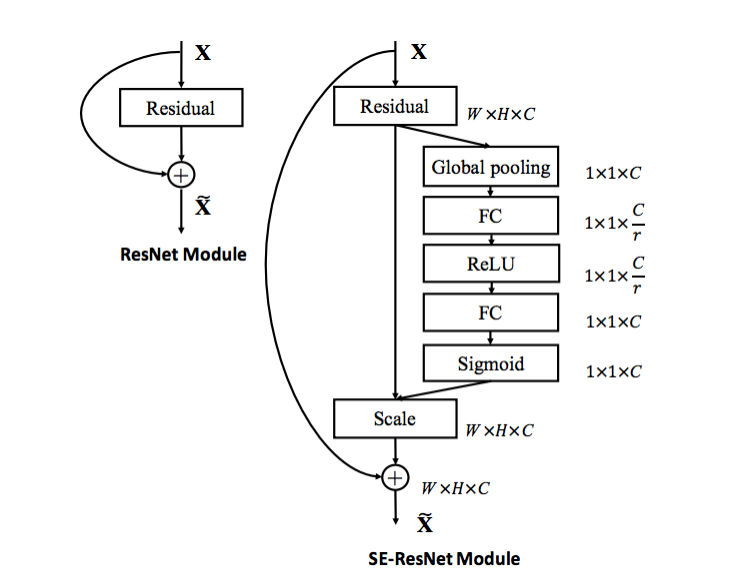
\includegraphics[scale=0.3]{./tex/attention-deep-learning/seres.png}
    \caption{Comparaison entre un module ResNet standard et un module SE-Resnet}
    \label{seres}
\end{figure}

\begin{figure}
    \centering
    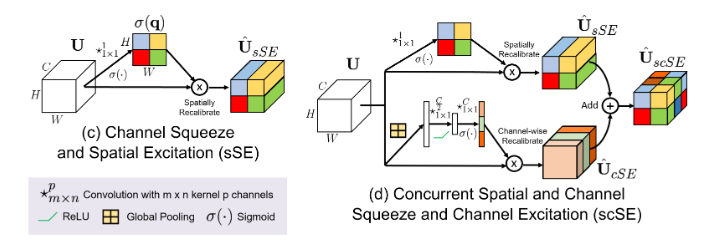
\includegraphics[scale=0.4]{./tex/attention-deep-learning/cse.png}
    \caption{Illustration des blocs sSE et scSE}
    \label{sse}
\end{figure}
